\chapter{Introduction}
\label{chap:introduction}
% -----------------------------------------------------------------------------

Ce projet a pour but d'aider l'institut ChemTech de la \acrshort{heia-fr} pour les recherches futures utilisant des liquides ioniques.
Ces liquides ioniques sont des éléments qui sont beaucoup utilisés en chimie.
Ils permettent notamment de stocker de l'énergie mais disposent aussi de nombreuses autres applications.

Les liaisons ioniques s'obtiennent par l'attraction de deux ions de charge opposée.
Les ions de charges positives et négatives sont respectivement appelés : cation et anion.
Généralement, les cations sont métalliques tandis que les anions ne le sont pas.
Un ion est composé d'un ou plusieurs atomes chargés électriquement.

Les possibilités de liaisons sont probablement infinies et leurs propriétés diffèrent pour chaque composition.
Dans notre cas, la particularité qui nous intéresse est le point d'ébullition.
Si on voulait obtenir cette information par expérience, il faudrait compter en jour le temps et les ressources consommées seraient importantes.
L'objectif de ce travail de semestre est d'estimer la température d'ébullition d'un liquide ionique afin de concentrer le temps et les ressources de l'institut ChemTech de la \acrshort{heia-fr} sur des liaisons validées par l'outil au préalable.

Ce travail sera utilisé comme outil de base pour un projet visant à stocker ou récupérer de l'énergie dans les phases de changements d'états d'un liquide ionique.
Le but est d'y insérer en entrée le \acrfull{smiles} de l'anion et du cation et d'en obtenir la température estimée.

L'écriture \acrshort{smiles} est utilisée en chimie pour décrire des molécules.
Cette écriture permet de reconstruire le modèle 3D ou 2D comme ci-dessous :
\begin{center}
   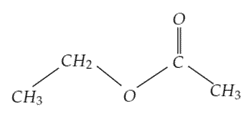
\includegraphics[height=20mm]{img/smiles_example.png}
   \captionof{figure}{Exemple de \acrshort{smiles}}
\end{center}

 
Il existe une librairie python qui permet de récupérer les informations issues d'un \acrshort{smiles}.

Ce projet a déjà été amorcé par Mme Yerly et Denis Marti, collaborateur effectuant son service civil à la \acrshort{heia-fr}.
Ils ont réussi à reproduire les résultats obtenus dans une étude\cite{WANG2021432} à l'aide de la base de données fournie par cette dernière et vérifier par la base de données de l'école.
Ce modèle était basé sur l'algorithme \acrfull{svm}.

Ces algorithmes ont besoin de données d'entrées et de cibles.
leur but sera de faire le lien entre les différents paramètres insérés et la cible la plus probable.

Dans un second temps, on pourrait aussi imaginer améliorer l'outil en rajoutant une surcouche qui déterminera le meilleur liquide ionique pour un objectif donné ou la possibilité de prédire d'autres propriétés.


\section{Objectifs}

Les Objectifs de ce projet sont découpés en deux catégories par niveau d'importance.


Les objectifs principaux consistent à reproduire les résultats de l'étude de Mme Yerly et de l'étudiant en master de mathématiques ainsi que regrouper et normaliser toutes les données nécessaires pour créer des modèles de \acrlong{ml}.
Le dernier objectif principale est le plus long et le plus intéressants car il faut créer un nouveau modèle à l'aide de l'écriture \acrshort{smiles}.


Les objectifs secondaires sont des améliorations qui pourraient être faites aux objectifs principaux.
Par exemple, nous avons la recherches de nouvelles données, le test de plusieurs algorithmes de \acrlong{ml} ou encore l'amélioration de l'\acrlong{ux}.
En effet, les interactions utilisateurs seront très sommaires et il y a beaucoup de chose envisageable comme une \acrshort{api}, un \acrshort{cli} ou une interface graphique.


\section{Activités}

Les activités sont découpées en 3 milestones. La première représente la phase de reproduction des résultats de l'étude de Mme Yerly et la mise en places des données normalisées.
La deuxième milestone représente la phase de création d'un nouveau modèle à l'aide de l'écriture \acrshort{smiles} et la troisième milestone représente la phase d'amélioration de l'outil.

Pour organiser le travail, j'utilise GitLab et le système d'épiques pour représenter le diagramme de Gantt.
Les avantages de ce systèm est que tout est centralisé à un seul endroit et le code peut être directement lié aux tâches, cependant la gestion de projet de GitLab a quelques désavantages comme par exemple, le diagramme de Gantt n'est pas très pratique à utiliser.

